\chapter{Background}
\label{cap:background}

% Maybe use "Background and State of the Art"

\section{Cyber Attacks}

% Terminologia, statisticas, tipos de ataques...

% 1 paragrafo contextualizando ataques nos anos de 2021 e 22. Detalhar ataques

% relatorios da symantec (olhar introdução do alexandre) ou da akamai

% HUMMEL, R.; HILDEBRAND, C. NETSCOUT Threat Intelligence Report - Issue 7: Findings From 1H 2021 - The Long Tail of Attacker Innovation. Westford, MA, USA, 2021. Retrieved on 2022-02-23. Available from Internet: <https://www.netscout. com/threatreport>.

\subsection{Attacks under study}


\section{Zeek Network Security Monitoring Tool}
\label{sec:bg:zeek}

An Intrusion Detection System, in our case for networks, is a system that monitors a network and is capable of generating alerts for network operators. These alerts help network operators to prevent future and ongoing cyber attacks. Currently, there are a number of different IDS solutions, which include Snort \cite{SnortWebsite}, Suricata \cite{SuricataWebsite}, and Zeek \cite{ZeekWebsite}. We focus on Zeek because of its open-source nature and architecture focused on extendibility and performance. Furthermore, it was the selected IDS for the by \citeonline{Ilha2022} for the original RNA, which is the basis of our proposed solutions in Chapters \ref{cap:rna} and \ref{cap:code_gen}.

Zeek is an Intrusion Detection System initially named Bro, which was proposed by \citeonline{Paxson1999}. Zeek is a passive IDS focused on high-speed monitoring, real-time notification and clear separation between mechanism and policy, and extensibility \cite{Paxson1999}. It was developed in a layered architecture shown in \autoref{fig:zeek_architecture}, which also enables the distribution of its processing to account for high throughput networks. The arrows represent incoming data, and dotted lines represent control and management communication. The first component of this architecture, from a bottom-up perspective, is the \textit{Packet Capture}. The \textit{Packet Capture} layer filters incoming packets from the network, ensuring only packets of interest reach the next layer, which is the \textit{Event Engine} (EE). The \textit{Event Engine} introduces semantic value to packets, translating them into events. The final layer, the \textit{Policy Script Interpreter} (PSI) receives the event stream, produced by the EE, and interprets these events, generating logs and sending real time alerts, or \textit{notices}, as Zeek calls them. We now dive into a bit more detail about each component.

\begin{figure}[htb]
    \caption{Zeek Architecture}
    \begin{center}
        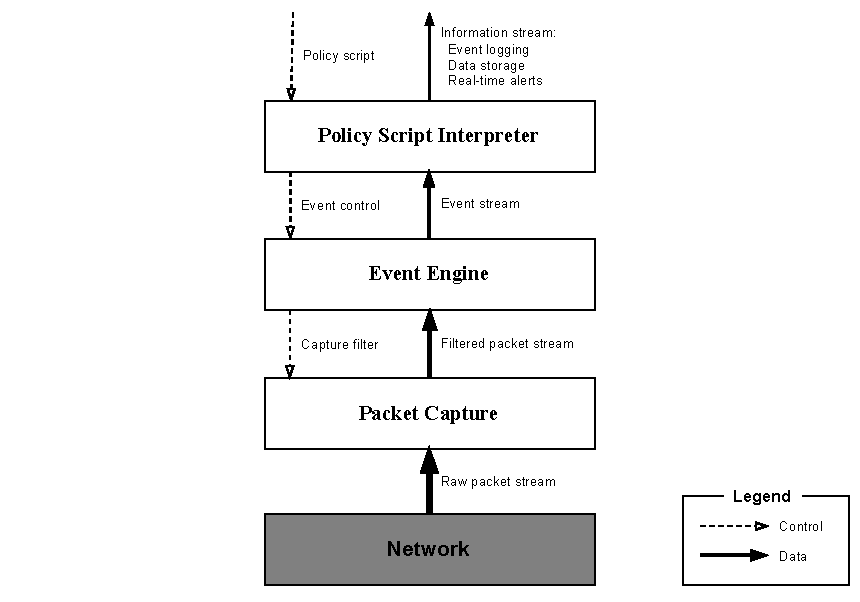
\includegraphics[width=1.0\textwidth]{images/zeek-architecture.pdf}
    \end{center}
    \label{fig:zeek_architecture}
    \legend{Source: \citeonline{Ilha2022}, adapted from \citeonline{Paxson1999}}
\end{figure}

\subsubsection*{Packet Capture}

The \textit{Packet Capture} layer was originally only conceived as the usage of the \textit{libpcap} library \cite{Libpcap}. It provides an abstraction layer between the network and the \textit{Event Engine}. With this extra layer, Zeek is isolated from network link layer technologies, enabling it to also read from packet traces saved as \textit{PCAP} files.

\subsubsection*{Event Engine}
\label{sec:bg:zeek_ee}

The \textit{Event Engine} is the most important layer for our Framework that is presented in \autoref{cap:rna}, and where our solution is executed. It's responsible for parsing incoming packets and generating events corresponding to those packets, for example, parsing an incoming ICMP Echo Request packet, and triggering the \texttt{icmp\_echo\_request} event with all the required structured information associated with it.

The internal structure of the \textit{Event Engine}, as explained by \citeonline{Ilha2022}, can be divided into four stages: acquisition, packet analysis, session analysis, and application layer parsing. In the acquisition stage, packets sent by the \textit{Packet Capture} component are received and forwarded to the next stage. In the packet analysis stage, the Packet Analysis Framework (PAF) receives the packets as Protocol Data Units (PDUs), and processes each layer of the packet. In this stage, where lower layer protocols are analyzed, there is still a clear definition of headers and payloads, and the headers usually contain the information of what is the next layer's protocol. Using this information, the PAF processes each header, extracting information and delivering its payload to the next layer until the transport layer. Each analysis layer in the Packet Analysis Framework is called an \textit{Analyzer}. This is important for later since this is where we add custom analyzers that will receive the custom messages from our Framework.

Still in the Event Engine, the session analysis stage creates a \textit{Connection} object that, despite the name, does not only represent a connection as in network terminology but also flows and sessions, for example, ICMP Echo Requests and Replies. This session is then stored and used to associate requests and replies, facilitating parsing for the next stage. After this \textit{session} has been created, the application layer parser selects possible application layer analyzers based on well-known port numbers. Since services are not strictly bound to specific ports, the application layer parser is able to dynamically identify application layer protocols using Dynamic Protocol Detection (DPD), which was introduced by \citeonline{Dreger2006}. Throughout the whole execution of the \textit{Event Engine}, it generates events that have semantic value, and that will be parsed by the PSI. These events vary from lower level events, such as a TCP connection established, with the \texttt{connection\_established} event, up to application layer protocols, for example, an FTP Request and Reply, represented respectively by the \texttt{ftp\_request} and  \texttt{ftp\_reply} events.


\subsubsection*{Policy Script Interpreter}
\label{sec:bg:zeek_psi}

The \textit{Policy Script Interpreter} is an event-driven script interpreter. It processes the events that were triggered by the \textit{Event Engine} using scripts written in a domain-specific language called Zeek. To process events, scripts define \textit{event handlers}, which are similar to functions, that process the events to generate logs and alerts. Zeek comes with multiple built-in scripts, such as FTP Bruteforce detection, traceroute detection, and others. Users can also write scripts and run their own policies.


\subsubsection*{Candidate Operations for Offloading}
\label{sec:bg:zeek_candidate_operations}



\section{Programmable Data Planes and the P4 Language}
\label{sec:bg:pdp}

A common miss-conception about Software Defined Networks (SDN) was about how programmable they were. While not entirely incorrect, this assumption revealed more complex probles as stated by \citeonline{Cordeiro2017}: Devices were programmable to a certain point, but developers were limited by a set of protocols and functions that were supported by the used ASICs (Application-Specific Integrated Circuit). Furthermore, OpenFlow API upgrades usually required hardware design changes to the ASICs, slowing down evolution of this technology. Programmable Data Planes (PDPs) emerged as a solution to these problems, allowing network operators to define protocols and network flow, effectively programming it. To program these devices, domain-specific languages (DSLs) were developed, two notable mentions are POF \cite{Song2013} and P4 \cite{Bosshart2014}. In this project, we focus on P4.


% \subsection{P4 Language}
\label{sec:bg:p4}

P4 stands for \textit{Programming Protocol-Independent Packet Processing}. It was proposed by \citeonline{Bosshart2014} and is a domain-specific language for programming network devices. P4 provides an abstraction for packet parsing and processing, by providing a generalized forwarding model \cite{Cordeiro2017}. It is also target independent and can be executed in different types of switches (fixed-function ASICs, NPUs, software switches, FPGAs).

To build P4's forwarding model, it is organized in three different sections: (a) \textit{data declaration}, (b) \textit{parser logic}, and (c) \textit{match+action tables and control flow} \cite{Cordeiro2017}. This structure can be seen on \autoref{fig:p4_model}. The \textit{data declaration} section defines all required data structures: the headers and the meta-data. These structures are mapped to a header and meta-data bus, which is used throughout the whole pipeline. The definition of P4 structure is similitar to \textit{struct} definitions in C, but are emphasized on bit sizes of all fields. The \textit{parser logic} specifies how packets are parsed and deparsed. This definition uses a state machine to define parsing states, progressing from one protocol to another. Finally, the \textit{match+action tables and control flow} defines the control flow of the ingress and egress pipelines. In this section, it is possible to define routing rules, and forward packets to a specific port. This is done using \textit{match+action} tables, which match specific header parameters to actions to be executed.

\begin{figure}[htb]
    \caption{P4 Forwarding Model}
    \begin{center}
        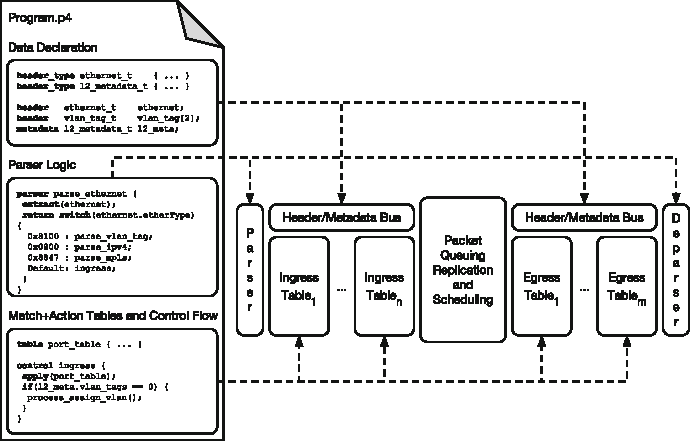
\includegraphics[width=1.0\textwidth]{images/p4model.pdf}
    \end{center}
    \label{fig:p4_model}
    \legend{Source: \citeonline{Cordeiro2017}, adapted from \citeonline{Kim2016}.}
\end{figure}

